\documentclass[a4paper, 12pt]{report}
\usepackage[top=1in,bottom=1in,left=1.5in,right=1in,headheight=0.5in,headsep=0.5in]{geometry}
\usepackage[utf8]{inputenc}                        % encoding document in uft 8
\usepackage{graphicx}                              % package for insertion of external images and other graphics formatting 
\usepackage{times}   
\usepackage{caption}                              % Times new roman font type
\usepackage{subcaption}                            % for captioning figures and labeling tables and equations
\usepackage{amsmath,amssymb,amsfonts}              % for mathematics symbols and fonts
\usepackage[hidelinks]{hyperref}                   % hyperref for inserting hyperlinks and hidelinks for hiding highlighting
\usepackage{cite}                                 % package for citation
\usepackage{float}                                % for different placement of figures and tables
\usepackage{enumitem}
\usepackage[british]{babel}
\usepackage{titletoc}                             % for table of contents, list of figures, list of tables.
\usepackage[nottoc,numbib]{tocbibind}             % for modifying table of content, nottoc removes toc from to
\usepackage[export]{adjustbox}   % package provides features for adjusting content within boxes,images, text, or tables. 
\usepackage{tabularray}
\usepackage{tabularx}
\usepackage{xstring}
\usepackage{algorithm}
\usepackage{algpseudocode}
\usepackage{microtype}


\begin{document}
\begin{center}
\thispagestyle{empty} %for removing page number in this page
\large{\bf{TRIBHUWAN UNIVERSITY \\ INSTITUTE OF ENGINEERING}}\\
\vspace{0.3cm}
\normalsize{\bf{Khwopa College of Engineering}} \\
\small{ Libali, Bhaktapur} \\
\normalsize{\bf{Department of Computer Engineering}} \\
\parskip 10mm

\includegraphics [width =30mm] {./img/Khwopalogo.jpg} \\
\vspace{0.3cm}
\normalsize{A Proposal \\ on} \\
\normalsize{\bf{Image Steganalysis Using Ensemble Classifiers  }} \\
\normalsize{\textit{Submitted in partial fulfillment of the requirements for the degree}}
\vspace{0.3cm} \\
\large{BACHELOR OF COMPUTER ENGINEERING}\\
\vspace{3.5cm}
Submitted by:\\
\begin{tabular}{p{0.5in}p{3.5in}p{3in}}
\hspace{0.3cm}&Sachin Koirala&KCE077BCT029\\
\hspace{0.3cm}&Sajal Poudel&KCE077BCT031\\
\hspace{0.3cm}&Unique Shrestha&KCE077BCT045\\
\hspace{0.3cm}&Utsav Chandra Kayastha&KCE077BCT046\\
\vspace{0.3cm}
\end{tabular}
\vspace{0.3cm} \\
\Large{\bf{Khwopa College of Engineering}}\\
\small{Libali, Bhaktapur}\\
\small{09 December 2023}
\end{center}


%\newgeometry{top=-1in,bottom=1in,left=1.5in,right=1in}

\begin{abstract}
\addcontentsline{toc}{chapter}{Abstract}
\thispagestyle{plain}
\pagenumbering{roman}
\setcounter{page}{1}
Steganography is a covert visual attack, that involves hiding malicious data inside innocent-looking carrier information. It's a technique for hiding information within an image, audio, or video file in such a way that the hidden information is not readily apparent to the human eye or ear. Digital images are the most common carrier format for steganography due to their frequent use on social media, websites, and email. Almost two-thirds of internet is made up of JPEGs, which serve as perfect carriers for these types of malware. Hence, it is important to have strong steganalysis methods. Our paper focuses on using ensemble classifiers as well as Generative Adversarial Networks (GAN) to detect hidden malicious contents in carrier files.  Ensemble classifiers is made up of various models working independently, employed to identify images modified using various steganography algorithms. These models are integrated into another model which utilizes algorithms such as logistic regression, to detect the presence or absence of malicious data. Generative Adversarial Networks (GAN) plays a crucial role in generating steganographically modified images, serving as a testing ground to ensure the effectiveness of the ensemble classifier models in successfully detecting and analyzing potential threats of steganogrpahically modified carriers. The core objective is to enhance steganalysis accuracy by integrating Machine Learning algorithms to counter the ever evolving field of steganography.
\end {abstract}

 
%\newgeometry{top=1in,bottom=1in,left=1.5in,right=1in}
\renewcommand{\contentsname}{Table of Contents}
\tableofcontents
\thispagestyle{empty}
\listoffigures
\listoftables
\clearpage
\addcontentsline{toc}{chapter}{List of Abbreviation}

\begin{flushleft}
    \Huge{\textbf{List of Abbreviation}}\vspace{1cm}\\
\end{flushleft}
\normalsize{\begin{tabular}{l l}
        GIF       & Graphics Interchange Format                \\
        JPEG      & Joint Photography Expert Group             \\
        PNG       & Portable Network Graphics                  \\
        bpnzac    & Bits Per non-zero                          \\
        J-Uniward & JPEG Universal Wavelet Relative Distortion \\
        DC-DM     & Distortion Compensated-Dither Modulation   \\
        ML        & Machine Learning                           \\
        PHARM     & Phase Aware Projection Model               \\
        DCT       & Discrete Cosine Transform                  \\
        UERD      & Uniform Embedding Revisited Distortion     \\
        CNN       & Convolutional Neural Network               \\
        DFT       & Discrete Fourier Transform\\
        FLD       & Fisher Linear Discriminant                 \\
        GFR       & Gabor Filter Residuals                     \\
        DCTR      & Discrete Cosine Transform Residuals        \\
        DOM       & Document Object Model                      \\
        DB        & Database                                   \\
        SQL       & Structured Query Language                  \\
        JSON      & JavaScript Object Notation                 \\
        API       & Application Programming Interface          \\
        RAM       & Random Access Memory                       \\
        GPU       & Graphics Processing Unit                   \\
        CUDA      & Compute Unified Device Architecture        \\
    \end{tabular}}


\chapter{Introduction}
\pagenumbering{arabic}
\section{Background}
Steganography is like hiding a secret message, like a picture or music. It's a way of keeping your message private by making it blend in, so others don't even realize there's a secret there. Steganalysis, the detection of hidden information within digital media, is crucial for maintaining the integrity and security of digital communication. Uncovering hidden information is vital for maintaining the security of digital communication channels, preventing covert communication that may pose risks.\vspace{0.5cm}\\
\textbf{Image Steganography}\\
Image Steganography is the process of hiding information which can be text, image or video inside a cover image. The secret information is hidden in a way that is not visible to the human eyes.
Different techniques of image steganography:
\begin{itemize}[noitemsep]
\item \textbf{nsF5}
\item \textbf{UERD(uniform embedding revisited distortion)}
\item \textbf{J-Uniward}\\
\end{itemize}
Steganography is an ever-evolving science of concealing information, continuously evolving to counteract detection methodologies. In response to this continuous evolution, the deployment of an automatically adaptive detection system becomes necessary. Embedding machine learning within steganalysis emerges as an optimal strategy to effectively counter the continuous evolution of covert communication methods.\\
\clearpage
\section{Problem Statement}
The continuous evolution of steganographic techniques poses a critical challenge to digital security. With the increasing sophistication of methods used to embed information covertly, traditional steganalysis approaches are challenged by the need for improved accuracy and adaptability. Since two-thirds of the internet is composed of images and images play a major role in digital communication, the use of advanced steganographic techniques to hide malicious data inside another carrier information poses an intricate threat to the security of a system. Creative approaches are required since secretly implanted malicious programs are difficult for traditional steganalysis to accurately identify. The complexity of compression and encryption methods adds an additional level of difficulty in detection. Existing steganalysis, which was created for traditional steganography, is not flexible enough to detect the ever-evolving algorithms for steganography. This proposal aims to fill these gaps by developing advanced machine learning-based steganalysis models that not only enhance accuracy and sensitivity but also exhibit adaptability to emerging steganographic trends. Thus, to protect the integrity of digital communication. This proposal seeks to propose an ever-evolving steganalysis process created with the help of ML to detect and tackle the subtle changes caused by the concealing of malicious data within unsuspecting carrier files.
\clearpage
\section{Objectives}
The main objectives of this project is to:
\begin{itemize}
\item \textbf{Adaptability to Emerging Techniques:} Develop steganalysis models that can adapt to emerging steganographic methods by continuously learning and updating their knowledge base.
\item \textbf{Algorithmic Innovation:} Explore novel algorithms and methodologies tailored to analyze the intricate patterns and structures associated with image-in-image steganography.
\item \textbf{Enhanced Feature Extraction}: Investigate and optimize feature extraction techniques to capture subtle anomalies indicative of image-in-image concealment, ensuring high detection accuracy.
\item \textbf{Adaptability to Diverse Image Formats:}Develop steganalysis models capable of detecting concealed images across a variety of image formats, resolutions, and compression methods.
\item \textbf{Benchmarking and Evaluation:} Establish a comprehensive benchmark dataset containing images with various steganographic content for testing and evaluating the performance of developed steganalysis techniques.
\item \textbf{Development of Specialized Steganalysis, Techniques:} Create and apply steganalysis methods with a particular goal in mind: identifying images that are hidden inside of another.
\item \textbf{Algorithmic Innovation:} Investigate modern techniques and algorithms designed specifically to examine the complex structures and patterns connected to image-in-image steganography.
Flexibility to Diverse Image Formats: Create steganalysis models that can identify hidden images in a range of image formats, compression techniques, and resolutions.
\item \textbf{Real-time Implementation:} Explore the integration of the developed models into real-time steganalysis systems. Evaluate their performance in dynamic environments.
\item \textbf{Benchmarking and Evaluation:} To test and evaluate the effectiveness of created steganalysis tools with photos that have different steganographic content.
\end{itemize}


\chapter{Literature Review} \hbadness=100000 \sloppy
Some work has been done in image steganalysis. Various steganalysis tools use different approaches like feature extraction, shallow ML, and deep learning methods to detect steganographically altered images. This literature review seeks to portray the history, methodologies, implementation and applications of steganalysis.\\
Multiple research has been done to achieve excellent results in steganalysis. Krzysztof Szczypiorski et al.\cite{1} used deep learning and ensemble classifiers to detect image steganography using different methods like DCTR and shallow machine learning classifiers. They found that performance depended heavily on the steganographic method used and on the density of the embedded hidden data. Detection of the content hidden with the nsF5 algorithm at the density 0.4 bpnzac was almost perfect while detection of data hidden using J-Uniward at 0.1 bpnzac was hardly possible. It is shown that steganalysis done using shallow ML is better in comparison to deep learning. This point is further proved by the fact that shallow ML consumes less resources and requires less time to be trained in comparison to deep ML and still provides accuracy similar or better than deep ML classifiers. \\
The document titled \textit{``The Discrete Cosine Transform: Theory and Application''}\cite{4} gives us a comprehensive overview of the Discrete Cosine Transform(DCT) and its application in digital image and video processing. The document discusses the properties of the DCT, including its decorrelation characteristics, energy compaction, and its ability to reduce entropy. It highlights the DCT's role in efficient coding and compression, particularly in the context of image and video standards such as JPEG and MPEG. Additionally, The document addresses the inverse DCT operation and its impact on visual distortion, providing examples of reconstructed images at different quantization levels.\\
\\George Berg et al.\cite{2} proposed an ML approach to steganalysis. This paper shows the feasibility of using a machine learning and data mining (ML/DM) approach to automatically build a steganography attack. This paper used three common data mining and learning techniques: decision trees, error back-propagation, artificial neural networks and the naïve Bayes classifier, to identify messages hidden in compression- (JPEG) and content based (GIF) images.\\
\\MT Hogan et al.\cite{3} evaluated the statistical limits by using probability density functions (pdfs). ML tests based on DC-DM are presented in this paper.To effectively uncover hidden information in images, we need a steganalysis tool with sharp pattern recognition skills. Sometimes, when we compare images that have been manipulated with certain tools to their original versions, we can spot a few noticeable visual irregularities – like odd pixels or changes in dimensions due to cropping or padding. If an image doesn't fit specific size criteria, it might get cropped or padded, and you'll see black spaces. Interestingly, most manipulated images don't give away obvious clues when compared to their originals. The simplest clue is a size increase between the manipulated and original images. Other signatures show up in how the colors are arranged in the image, such as a significant change in the number of colors or a gradual increase or decrease. Grayscale images follow a different pattern, increasing incrementally. Another strong indicator is an unusual number of black shades in a grayscale image.\\
\textit{``Steganalysis in high dimensions: Fusing classifiers built on random subspace''}\cite{8} provides core concepts of this project such as ensemble classifier and importance of selection of features. A distinctive subject which it has touched upon is the concept of Curse of Dimensionality (CoD) which shows the relation of complexity and increase in  resource usage for computation. It is highlighted how ensemble classifiers can counter this problem by using reduced dimension for training its base learners.\\
\textit{``Ensemble Classifiers for Steganalysis of Digital Media''}\cite{5} highlights several key studies in the field of steganalysis, which provides a solid foundation for understanding the current state of steganalysis. The document discusses the implementation of ensemble based steganographically altered image classifier using many base learners for classification. The proposed base learners are trained using FLD analysis due to its ability to increase diversity The performance of the proposed model even though gets trained in very less time in comparison to usually used classification method of G-SVM can classify with similar or better accuracy. It is highlighted that a G-SVM classifier takes about 8 hours to be properly trained while an ensemble classifier takes only 20 minutes.\\                   
\textit{``A fast and accurate steganalysis using Ensemble classifiers''}\cite{6} provides an in-depth insight into the use of an ensemble of classifiers for steganalysis, with a focus on machine learning. The ensemble-based steg analyzer uses feature vectors from multiple stegalyzers to create a decision algorithm that allows the combination of information from different steganalyzers. The resulting steganalyzer is also inherently suitable for multi-class classification scenarios. The paper presents a novel steganalysis decision framework using hierarchical classifiers, which addresses the limitations of existing steganalysis methods and provides a scalable and cost-effective approach to steganalysis. Ensemble classifiers are designed to overcome the limitations of individual classifiers by combining their outputs to achieve better performance. Steganalysis using ensemble classifiers is a powerful approach that utilizes the strength of multiple classifiers to help improve the detection of hidden information in images. It provides diverse steganographic techniques while also enhancing the overall accuracy. Ensemble classifiers are designed to overcome the limitations of individual classifiers by combining their outputs, thereby achieving better performance.\\
\textit{``J. Kodovský and J. Fridrich. Calibration revisited''}\cite{9} provide information on the pre features and their Cartesian calibrated and Non-cartesian calibrated form.``A Markov Process Based Approach to Effective Attacking JPEG Steganography''\cite{10} and ``Merging Markov and DCT features for multi-class JPEGsteganalysis''\cite{11}  guides the outlook of our project to a better angle as it provides very crucial details on the section of feature extraction.They provide more insight on the pre features which can be utilized for better classification. These literature provided more insights on CC-PEv and CC-SHI which are different pre features used for steganalysis. “JPEG Image Steganalysis Utilizing both Intrablock and Interblock Correlations”  provides more insight on the importance of considering relation between inter and intra block correlations during pre feature creation for better detection or classification. \\
The dataset we will be using on this project will be taken from IStego100k\cite{7}. IStego 100K is a large-scale steganalysis consisting of 208,104 images with a size of 1024*1024 pixels. The training set consists of 200,000 images organized into 100,000 cover-setgo image pairs. The testing set comprises the remaining 8,104 images. Each image in the dataset has randomly assigned quality factors in the range of 75-95. Three well-known steganographic algorithms J-uniward, nsF5, and UERD\cite{}\cite{12}\cite{13} are randomly selected for embedding in the images. The embedding rate for each image is randomly set in the range of 0.1-0.4 bpac.\\ 
\\The relevant papers that we studied to grab knowledge about this project are given in the review matrix below:
\begin{table}[!h]
        \begin{tabular}{|p{0.7cm}|p{3cm}|p{0.8cm}|p{3cm}|p{1.3cm}|p{3cm}|}
            \hline
        S.N. & Name                                                                            & Year & Authors                                                                                & Dataset          & Findings                                                                                                                                                                                          \\\hline
        1    & Searching for hidden messages Automatic detection of steganography              & 2003 & George Berg, Ian Davidson, Ming-Yuan Duan, and Goutam Paul                            & BOSS             & Images are commonly used to transmit hidden messages. Different strategies are used to hide messages in GIF and JPEG formats.                                                                     \\\hline
        2    & International Workshop on Information Hiding                                    & 2005 & Jessica Fridrich, Miroslav Goljan, and David Soukal                                    & NA               & NA                                                                                                                                                                                                \\\hline
        3    & On steganographic embedding efficiency                                          & 2007 & Jessica Fridrich, Petr Lisonek, and David Soukal.                                      & NA               & NA                                                                                                                                                                                                \\\hline
        4    & Ml detection of steganography                                                   & 2005 & Mark T Hogan, Neil J Hurley, Guenole CM Silvestre, Felix Balado, and Kevin M Whelan    & BOSS             & NA                                                                                                                                                                                                \\\hline
        5    & The discrete cosine transform (dct) theory and application                      & 2003 & Syed Ali   Khayam.                                                                     & NA               & NA                                                                                                                                                                                                \\\hline

        \end{tabular}
\end{table}
\clearpage
\begin{table}[!h]
    \begin{tabular}{|p{0.7cm}|p{3cm}|p{0.8cm}|p{3cm}|p{1.3cm}|p{3cm}|}
        \hline
    S.N. & Name                                                                            & Year & Author                                                                                 & Dataset          & Findings                                                                                                                                                                                          \\\hline
    6    & Steganalysis in high dimensions Fusing classifiers built on random subspaces    & 2011 & Jan Kodovsky and Jessica Fridrich.                                                     & BOSS             & The paper proposes ensemble classifiers as an alternative   to support vector machines. Experiments with steganographic algorithms nsF5   and HUGO demonstrate the usefulness of this approach.   \\\hline
    7    & Ensemble classifiers for steganalysis of digital media                          & 2012 & Jan Kodovsky, Jessica Fridrich, and Vojtech Holub.                                     & BOSS             & Ensemble classifiers have improved detection accuracy for steganographic methods in JPEG images. The proposed framework allows for fast construction of steganography detectors.                  \\\hline
    8    & Proceedings of the 11th ACM Workshop on Multimedia and Security                 & 2009 & Jan Kodovsky and Jessica Fridrich.                                                     & NA               & NA                                                                                                                                                                                                \\\hline
        9    & Merging markov and dct features for multi-class jpeg steganalysis               & 2007 & Tomas Pevny and   Jessica J. Fridrich                                                  & BOSS             & The paper   constructs a new multi-class JPEG steganalyzer with improved performance. The   new feature set provides significantly more reliable results compared to   previous work.             \\\hline
    \end{tabular}
\end{table} 
\clearpage
    \begin{table}[!h]
        \begin{tabular}{|p{0.7cm}|p{3cm}|p{0.8cm}|p{3cm}|p{2cm}|p{3cm}|}
            \hline  
            S.N. & Name                                                                            & Year & Authors                                                                                & Dataset          & Findings                                                                                                                                                                                          \\\hline
    10   & Detection of image steganography using deep learning and ensemble classifiers   & 2022 & Mikołaj Płachta, Marek Krzemien, Krzysztof Szczypiorski, and Artur Janicki             & BOSS             & Ensemble classifiers performed well in steganography detection. Deep learning algorithms achieved better results for UERD and nsF5 steganographic algorithms.                                     \\\hline
    11   & A markov process based approach to effective attacking jpeg steganography       & 2007 &Yun Q. Shi, Chunhua Chen, and Wen Chen.                                                 & BOSS             & The proposed steganalyzer outperforms  by a significant margin. The detection rates are higher while considering the introduced features.                                                         \\\hline
    12   & A fast and accurate steganalysis using ensemble classifiers                     & 2013 & Arezoo Torkaman and Reza Safabakhsh                                                    & BOSS             & The proposed method achieved a lower error rate of 46\%   compared to the ensemble classifier. The training time of the proposed method   was 88\% lower than the ensemble classifier.            \\\hline
    13   & Istego100k   Large-scale image steganalysis dataset                             & 2019 & Zhongliang Yang, Ke Wang, Sai Ma, Yongfeng Huang, Xiangui Kang, and Xianfeng Zhao      & IStego100K      & The paper introduces a large-scale image steganalysis dataset called IStego100K. The performance of some steganalysis algorithms on IStego100K is tested.                                        \\ \hline                   
        \end{tabular}
    \caption{Review Matrix with Research Papers, authors and purpose}
\end{table}


    

\chapter{Feasibility study}
After the problem is clearly understood and solutions proposed, the next step is to conduct the
feasibility study. Feasibility study is defined as evaluation or analysis of the potential impact
of a proposed project or program. The objective is to determine whether the proposed system
is feasible. There are three aspects of feasibility study which are discussed below.\\
\hbadness=99999 
\textbf{Technical Feasibility:}\\For the technical part, we're getting our project data from the Kaggle and BOSS datasets which contain various datasets containing stenographically modified images. These images have been modified using different algorithms which creates diversity in the dataset used improving the reliability of the system. We're using free software to build the project, and the department is providing cloud resources like RAM and GPU for training our model. This setup makes sure our project is doable and integrates well with the currently existing system. Thus, we can conclude that it is technically feasible.\\
\textbf{Economical Feasibility:}\\The only cost for the project is the computational power, covering processing and electricity. Since the department will be providing the processing power needed to train the model, the cost is almost zero. Therefore, this project is economically viable.\\
\textbf{Operational Feasibility:}\\We have decided to use the Shallow ML approach which allows the model to be trained with less computational power in comparison to deep learning. For shallow machine learning we are planning to implement an ensemble classifier and each of its models will be trained using FLD to improve its effectiveness. Deep learning implements the CNN approach which requires higher computational power to be trained. Thus, we decided to use a simpler machine learning approach that doesn't need a lot of computational power, unlike the more complex deep learning method called Convolutional Neural Network (CNN). After we train the system, it's ready to use and can easily be added to a webpage or any other interface. This way, the system is practical and doesn't need a lot of resources making it able to be effectively implemented in real-life applications. Thus, it is operationally feasible.
\\
\chapter{Methodology}
\section{Software Development Approach}
 is an iterative process-based approach to software development. In the Agile process model, work is broken down into more manageable, smaller iterations without requiring a lot of long-term planning. The requirements and scope of the project are determined early on, and the number, length, and scope of each iteration are preplanned. Each iteration is considered as a short time "frame" in the Agile process model, which lasts for a few weeks. In each iteration, teams move through the phases of the software development life cycle, which include planning, requirements analysis, design, coding, testing, and demonstration of a working product for client review. Agile places a significant value on flexibility, teamwork, and regular client feedback.\\
\begin{figure}[H]
    \centering
    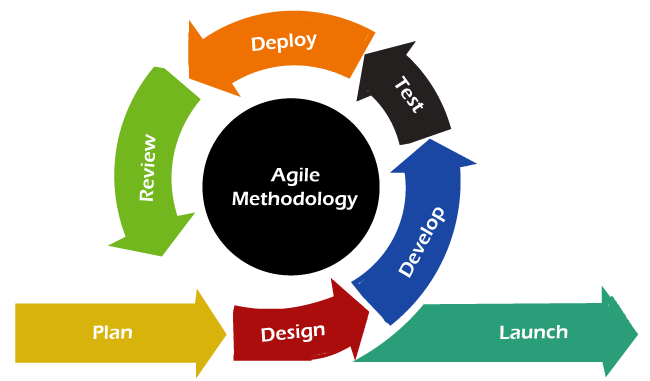
\includegraphics[width=80mm]{./img/agile.png}
    \caption{Agile Model}
\end{figure}
The main reason for which  we choose this development process:
\begin{enumerate}[noitemsep] %label=\Roman*.]
\item Very quick,flexible and efficient.
\item Risk minimization.
\item Projects are split into sprints for better management and productivity.
\item Through iterative testing and sprints, the final product contains less bugs. 
\item Development period for application is reduced.
\end{enumerate}
\begin{figure}[H]
\section {Block diagram of proposed system}
% \centering
                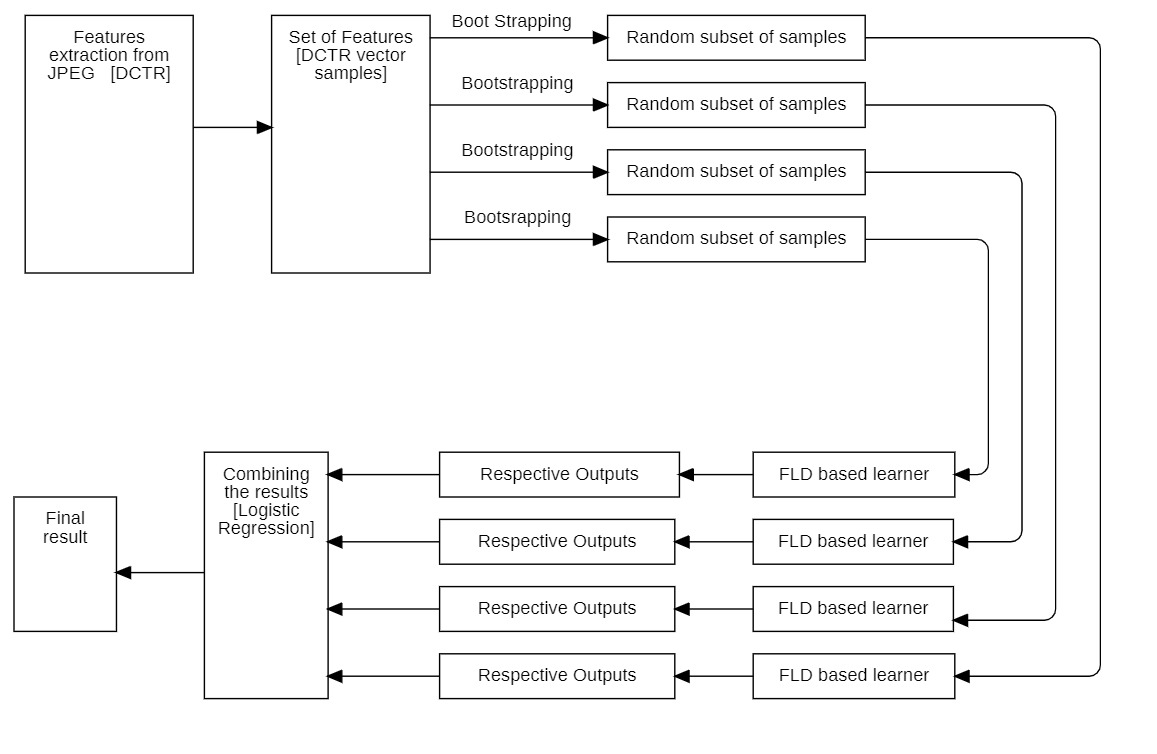
\includegraphics[width=1.1\textwidth]{./img/block_d.jpg}\\
\caption{ Block diagram of proposed system}
\end{figure}
\clearpage

\begin{flushleft}
    \Large{\textbf{Model Training Approach}}\\
\end{flushleft}
\textbf{Feature Extraction:}\\
Initial extraction of DCTR (Discrete Cosine Transform Ratio) feature vector from images or.jpeg files is to be done. The selection of DCTR is based on its detection efficiency in comparison to other parameters such as PHARM and GFR.\vspace{0.25cm}\\
\textbf{Ensemble Classifier Selection:}\\
The decision to choose ensemble classifiers over deep learning techniques was made due to their superior steganalysis detection efficiency and their need for lesser computational power.\vspace{0.25cm}\\
\textbf{Bootstrapping:}\\
Bootstrapping is the process of splitting a large dataset into its smaller subsets. The gathered DCTR feature vectors are to be split  into more manageable subsets. Utilizing these subsets, individual base models are to be trained independently.\vspace{0.25cm}\\
\textbf{Base Learner Training:}\\
Based on the extracted features, each base learner independently processes its subset of feature vectors and finalizes a decision.\vspace{0.25cm}\\
\textbf{Aggregation:}\\
To create an ensemble decision, the choices made by each individual base learner are aggregated and the final decision is to be made by using a voting system which finalizes the result by figuring out the most popular output.\vspace{0.25cm}\\
\textbf{Efficiency Considerations:}\\
The proposed system prioritizes efficiency by leveraging shallow machine learning techniques, particularly ensemble classifiers instead of deep learning. The choice of DCT as a feature is intentional to increase efficiency and detection capability of the system.\\
\clearpage 

\section{Description of working flow of proposed system}
\begin{figure}[H]
    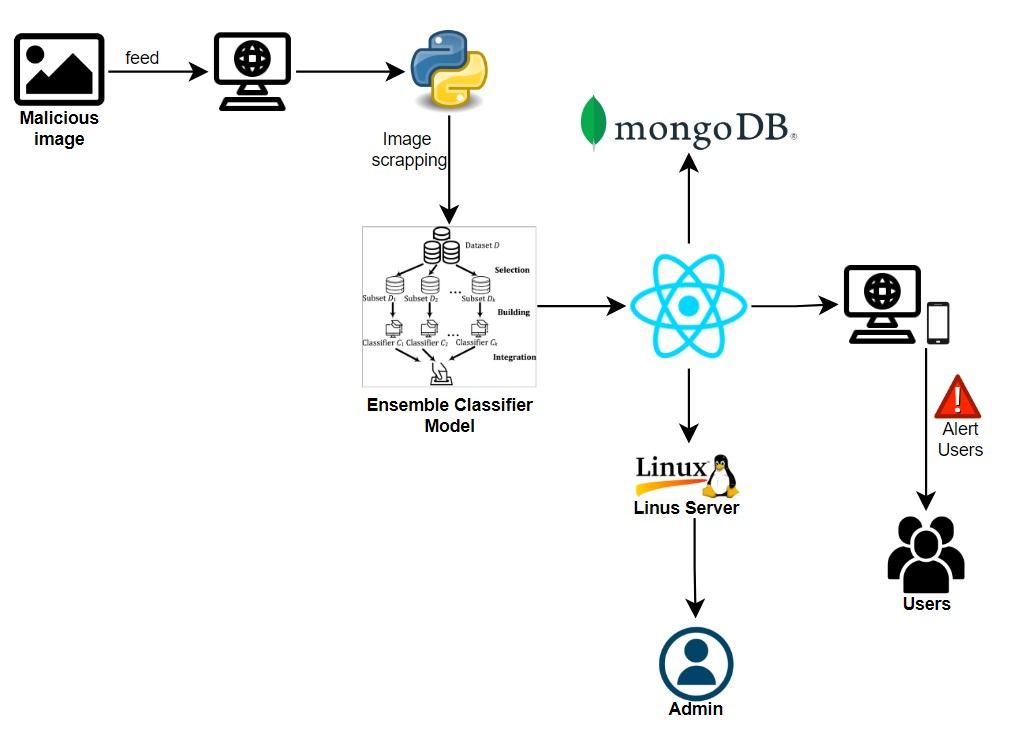
\includegraphics[width=180mm]{./img/System architecture.jpg}
    \caption{System Architecture}
\end{figure}
\clearpage 

\chapter {Implementation Plan}
\section{Gantt Chart}
\begin{figure}[H]
        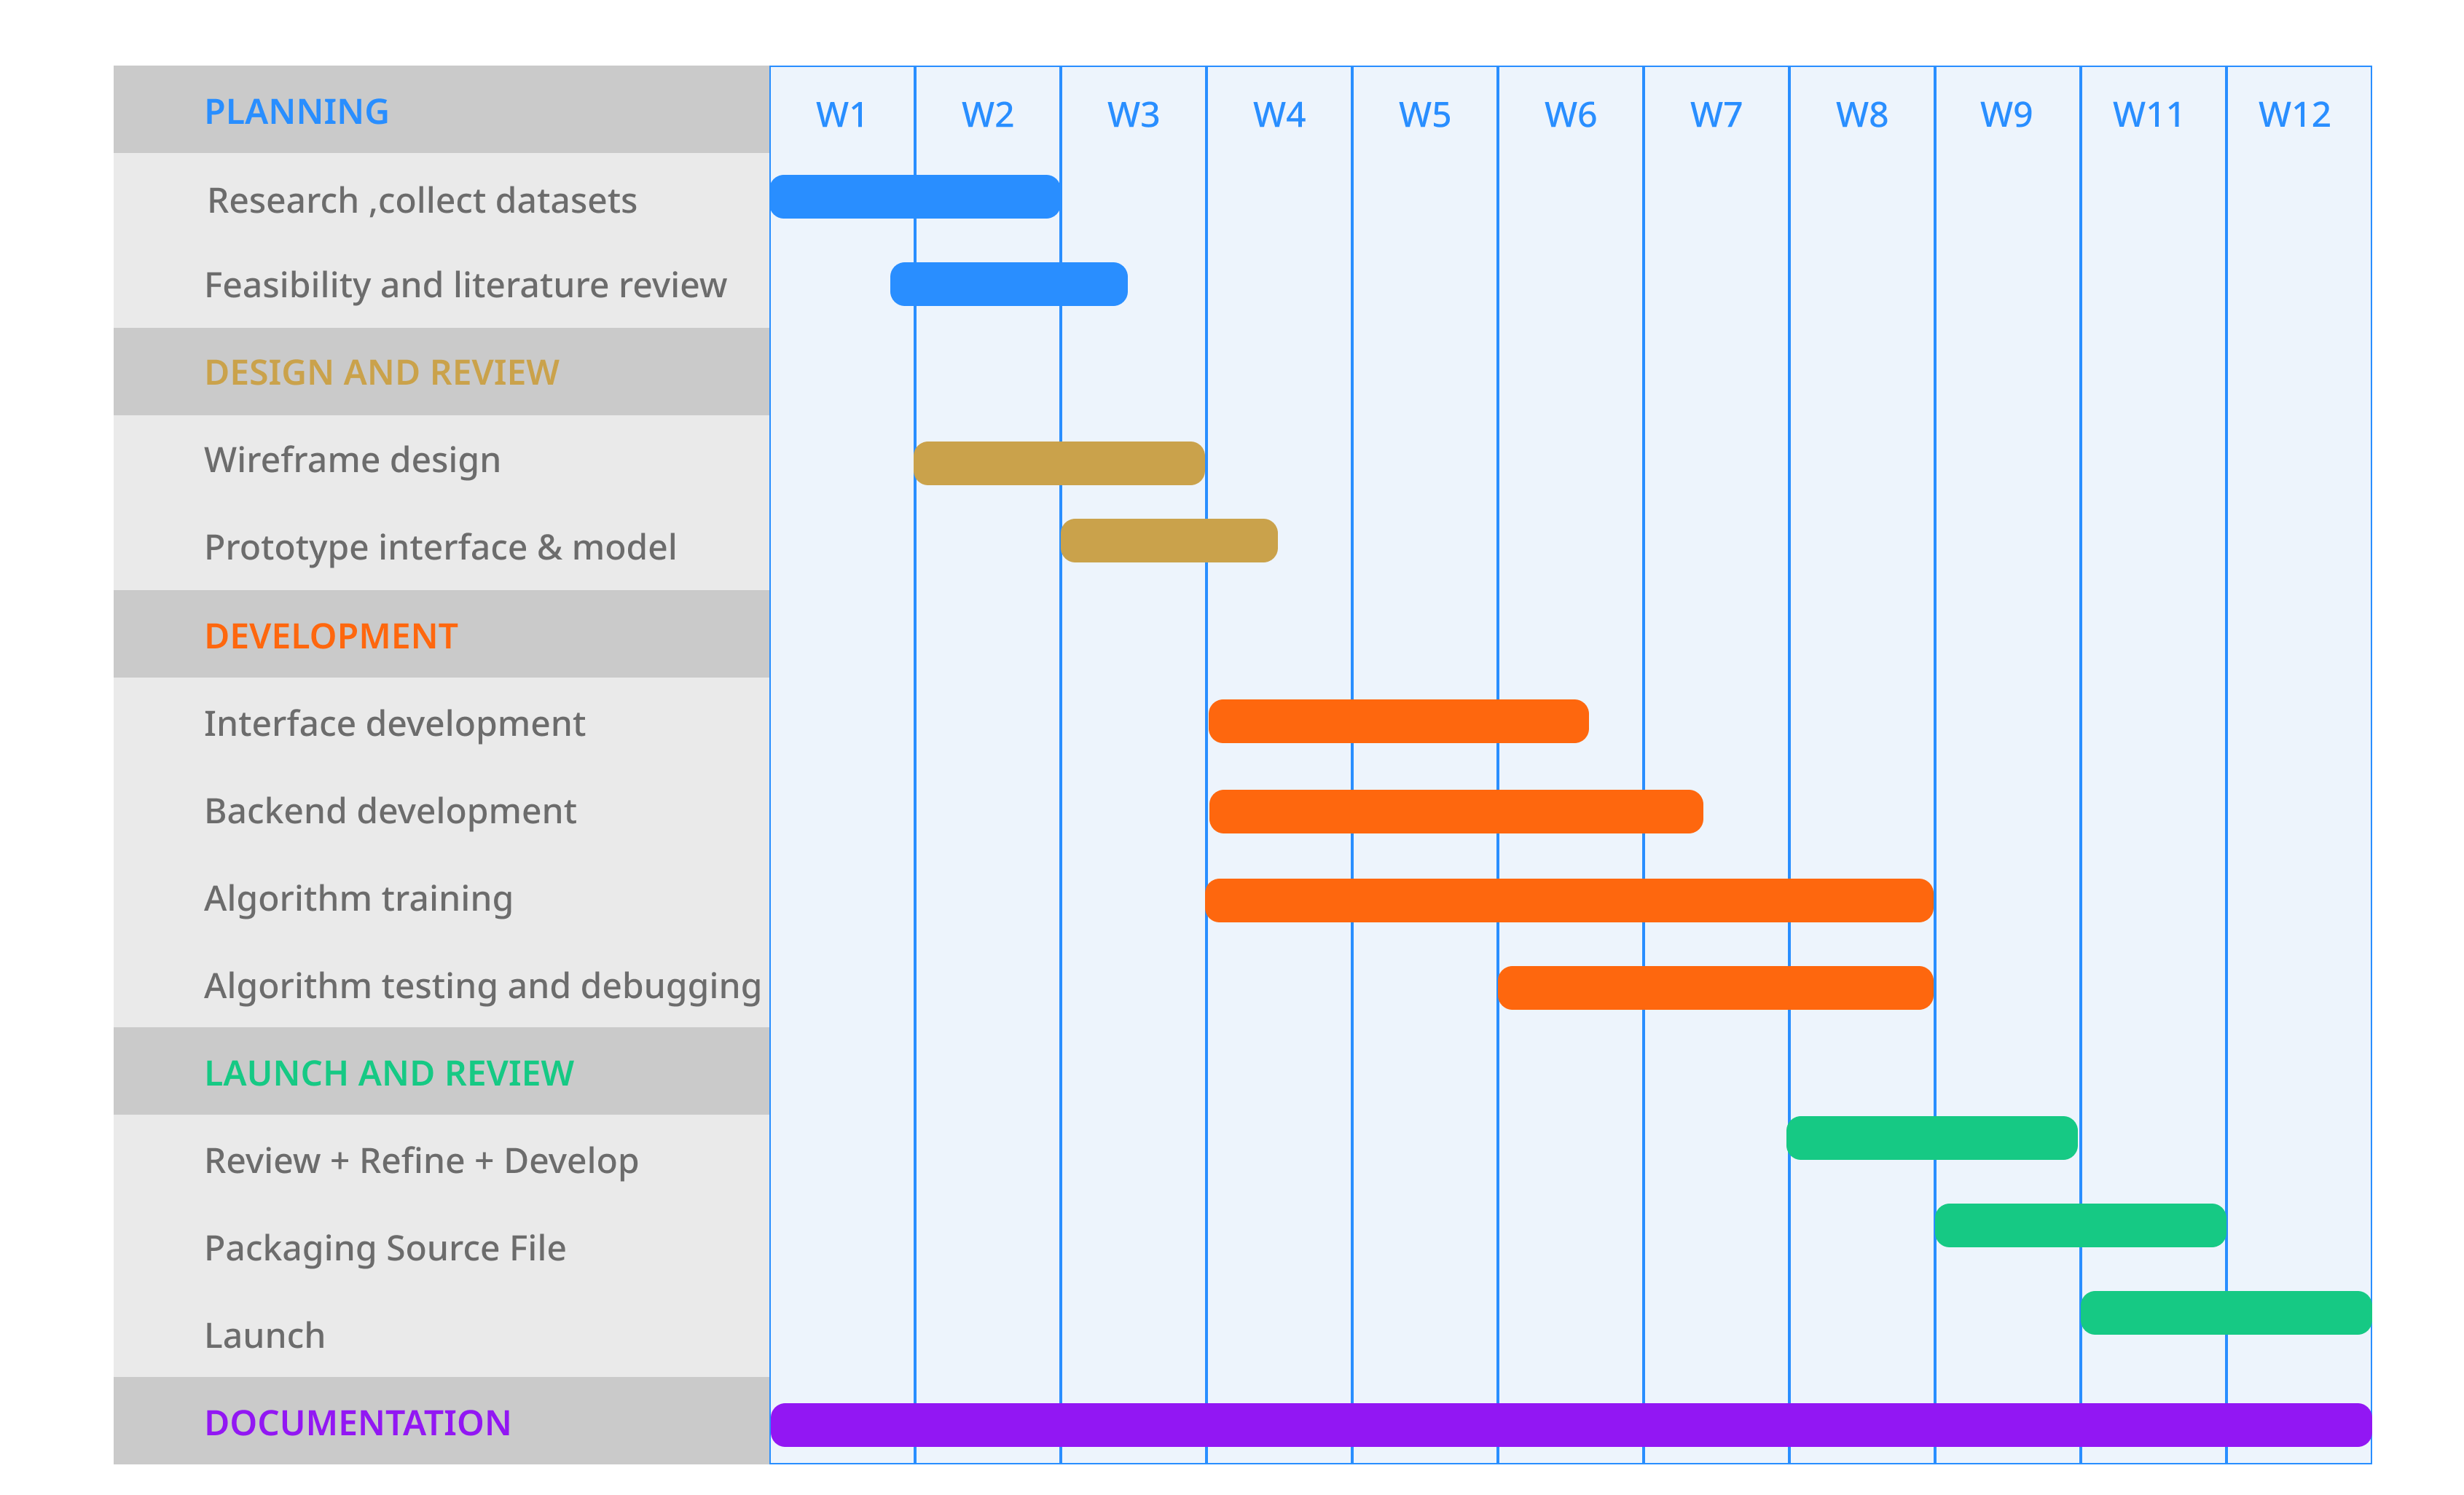
\includegraphics[width=150mm, left]{./img/gantt_chart.png}
\caption{Gantt Chart}
\end{figure}
\clearpage
\section{Software Requirement}
\begin{itemize}[noitemsep]
\item \textbf{Python:} 
Python is a versatile programming language commonly used for developing software applications. It can be used for various tasks in the system, such as backend development, data processing, and machine learning integration.
\item \textbf{MongoDB:}
MongoDB is a widely used NoSQL database, utilizes JSON-like documents for data storage, ensuring excellent performance and scalability. Its schema-less structure supports dynamic data modeling, making it well-suited for web applications. By employing collections instead of conventional tables and incorporating horizontal scaling, MongoDB efficiently handles diverse data types across multiple servers. This versatility positions it as a robust solution for contemporary, data-driven environments.
\item \textbf{React }
 React is a JavaScript library for building user interfaces, particularly in single-page applications. Developed by Facebook, it uses a declarative approach for efficiently updating the DOM. With a component-based structure, React enhances modularity and reusability, making it a popular choice for creating interactive and scalable web applications.
\item \textbf{Javascript:}
JavaScript is a programming language commonly used for developing web-based applications. It can be used for front-end development, implementing interactive features on the system’s web interface, and facilitating communication with the backend. 
\item \textbf{Tensorflow: }
TensorFlow is an open-source machine-learning framework that provides a wide range of tools and libraries for building and deploying machine-learning models. It can be used for image recognition, object detection, and prediction algorithms in the Smart Parking Management System.
\item \textbf{Keras:}
Keras is a high-level neural networks API written in Python. It can be used as a user-friendly interface to TensorFlow, simplifying the process of designing and training deep learning models for tasks like number plate recognition or image analysis in the system.
\item \textbf{VS Code:}
VS Code is a popular and widely used source code editor that offers a range of features and extensions to enhance the development experience. It supports multiple programming languages, including Python, JavaScript, and React, making it suitable for working with the different components of the system. 
\end{itemize}


\section{Hardware Requirement}
\begin{enumerate}[noitemsep] %label=\Roman*.]
   \item High dedicated RAM to handle memory-intensive tasks
   \item NVIDIA GPU for optimal performance.
   \item Dedicated GPU with CUDA support for accelerated parallel processing.
   \item  SSD storage for faster read/write speeds during image processing.
   \item Additional high-capacity external storage for storing large datasets and image collections.
   \item Smartphone or tablet for testing mobile applications  
\end{enumerate}

\chapter{Expected Outcomes}
The proposed system is expected to detect stego images using ML model. It would be capable of decting hidden information with high accuracy. It is expected to be able to identify and optimize the extraction techniques to improve the sensitivity and specificity of steganalysis. The model will be able to adapt to emerging steganographic techniques and provide real-time dection capabilities. 







\bibliographystyle{unsrt}  
\bibliography{ref}
\end{document}

